\section{Archived Static Stitching Evaluation}
\label{sec:legacy-evaluation}
We evaluate saved software outputs from the calibrated panorama pipeline
and three image-based baselines. This is an analysis of existing outputs, not a new run of
the renderers or neural networks. Its scope is pre-blend photometric consistency
between warped views of this calibrated rig; it does not measure temporal
stabilization, absolute gravity alignment, or the integrated FPGA output.

\subsection{Cases, Configurations, and Metrics}
The archive contains six named EO cases with six source views. The StabStitch++ wrapper evaluates cameras 0--2. We therefore use a
shared target set of 12 case/pair identities for all four methods: pairs
$(0,1)$ and $(1,2)$ in each case. The wraparound pair $(5,0)$ is outside this evaluation. The six case names
identify configurations; they do not establish six statistically independent
scenes or acquisitions.

The saved UDIS++ configuration requests 30 iterations of per-pair adaptation,
and the associated code contains optimizer updates \cite{nie2023parallax}.
StabStitch++ is supplied with 16 repetitions of each static input image to
satisfy the temporal interface \cite{nie2025stabstitch2}. Its results here
therefore test static alignment under that wrapper, not its video-stability
capability. The preparation script undistorts the image-based inputs using
the recorded intrinsics. The calibrated renderer additionally uses mounting
geometry and inertial angles, so the methods still receive different priors.

We preserve the archived metric formula. Images are converted to grayscale;
the overlap mask is eroded by a $5\times5$ square. PSNR and the mean local SSIM
map \cite{wang2004ssim} are evaluated over that mask, both directly and after
Gaussian smoothing with $\sigma=2$ output pixels. We call the latter
\emph{smoothed} scores, not independent measures of geometric error. Each
reported mean weights case/pair identities equally. The calibrated renderer,
UDIS++, and StabStitch++ scores are recomputed from saved warped images; SIFT
scores are retained from the saved evaluator JSON, which used its original
in-memory masks.

This protocol has material limitations. The calibrated renderer infers validity
from image intensity, whereas the baselines use saved masks. Output scales,
canvases, compression, and visible regions differ, so Gaussian smoothing with
$\sigma=2$ pixels does not represent a shared angular scale. Exposure, texture, parallax,
and smoothing affect both metrics. Consequently these scores describe the saved
outputs under their original evaluation conventions; they are neither
ground-truth registration errors nor a controlled ranking of the methods.

\begin{table}[t]
\centering
\caption{All 12 shared target identities. Scores are means over each method's
successful outputs; raw/smoothed values are separated by a slash. The SIFT row
has a different successful subset and is not directly comparable as a paired
mean. Different masks and scales remain throughout.}
\label{tab:legacy-targets}
\small
\setlength{\tabcolsep}{3pt}
\begin{tabular}{lccc}
\toprule
Method & Valid/target & PSNR (dB) & SSIM \\
\midrule
Calibrated G-locked & 12/12 & 15.05/22.59 & .311/.752 \\
UDIS++ & 12/12 & 13.47/16.88 & .205/.424 \\
StabStitch++ & 12/12 & 12.82/15.56 & .213/.450 \\
SIFT + homography & 9/12 & 13.24/16.16 & .304/.534 \\
\bottomrule
\end{tabular}
\end{table}

\subsection{Matched Identities and Retained Failures}
Table~\ref{tab:legacy-targets} reports coverage before any common-success
selection. The SIFT evaluator records failures for case
\texttt{EO\_Test2\_R\_2.15\_P\_0}, pair $(0,1)$;
\texttt{EO\_Test5\_R\_4.75\_P\_-4.5}, pair $(1,2)$; and
\texttt{EO\_Test6\_R\_1.25\_P\_6.5}, pair $(0,1)$.
We retain these failures explicitly instead of assigning an arbitrary metric
value or treating absent scores as successful measurements.

Figure~\ref{fig:legacy-matched} restricts all four methods to the nine identical
case/pair identities with available successful scores. Smoothed PSNR/SSIM are
$22.56$/.757 for G-locked, $17.09$/.442 for UDIS++, $15.60$/.466 for
StabStitch++, and $16.16$/.534 for SIFT. G-locked has higher recorded values on
this conditional subset. Matching identities controls the sampled camera pairs, but not the mask,
scale, or information differences described
above. These descriptive means do not support statistical significance or
generalization claims. No IR baseline runs were found in this comparison
archive, so it cannot establish comparative IR generalization.

\begin{figure}[t]
\centering
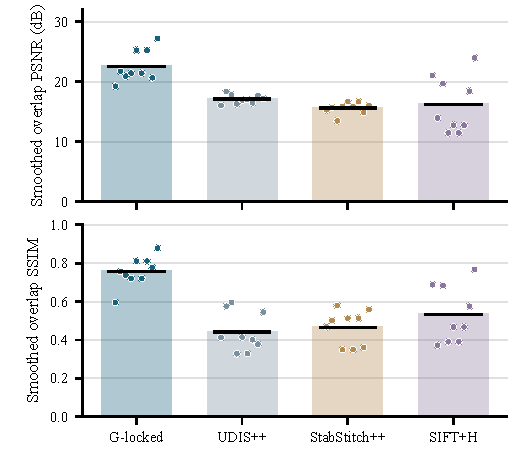
\includegraphics[width=\columnwidth]{figures/legacy_matched_comparison.pdf}
\caption{Saved-output comparison on nine common-success case/pair identities;
dots represent individual pairs and horizontal lines their means.
Coverage is reported against the 12-target set. Masks, output scales, and
calibration access differ across methods. These conditional photometric scores
do not measure temporal stabilization or independent geometric accuracy.}
\label{fig:legacy-matched}
\end{figure}

The accompanying reanalysis script, per-seam CSV, and JSON manifest record
target identities, failures, software versions, source-file hashes, and the
metric conventions. They reproduce the summary when the identified local
archive is supplied; the raw captures and original model runs are not included
in this paper repository. The next evaluation step is to use independently
measured geometry and synchronized dynamic captures, with common output scale,
validity support, and a declared adaptation budget.
